\documentclass{article}
\newtheorem{thm}{Theorem}
\setlength{\oddsidemargin}{0.25in}
\setlength{\textwidth}{6in}
\setlength{\topmargin}{-0.25in}
\setlength{\headheight}{0.3in}
\setlength{\headsep}{0.2in}
\setlength{\textheight}{9in}
\setlength{\footskip}{0.1in}
\usepackage{multirow}
\usepackage{fullpage}
\usepackage{graphicx}
\usepackage{amsthm}
\usepackage{amssymb}
\usepackage{url}
\usepackage{amsfonts}
\usepackage{algpseudocode}
\usepackage{mathtools}

\usepackage{listings}
\usepackage{color}
 
\definecolor{codegreen}{rgb}{0,0.6,0}
\definecolor{codegray}{rgb}{0.5,0.5,0.5}
\definecolor{codepurple}{rgb}{0.58,0,0.82}
\definecolor{backcolour}{rgb}{0.95,0.95,0.92}
 
\lstdefinestyle{mystyle}{
    backgroundcolor=\color{backcolour},   
    commentstyle=\color{codegreen},
    keywordstyle=\color{magenta},
    numberstyle=\tiny\color{codegray},
    stringstyle=\color{codepurple},
    basicstyle=\footnotesize,
    breakatwhitespace=false,         
    breaklines=true,                 
    captionpos=b,                    
    keepspaces=true,                 
    numbers=left,                    
    numbersep=5pt,                  
    showspaces=false,                
    showstringspaces=false,
    showtabs=false,                  
    tabsize=2
}
 
\lstset{style=mystyle}

\begin{document}\title{Project 6: Test Search Engine\\ Cloud Computing\\ Spring 2017}         % Enter your title between curly braces
\author{Professor Judy Qiu }        % Enter your name between curly braces
\date{}
%\date{\today}          % Enter your date or \today between curly braces
\maketitle
\makeatother     % `@' is restored as a "non-letter" character
\pagestyle{plain}
\section*{Goal}
After having familiarized yourself with the ``HBase Building an Inverted Index'' homework and ``PageRank algorithms'' homework, you are ready to use these applications to test the search engine function from the packaged executable.

\section*{Deliverables}
Zip your source code, library, and results in a file named username@test-search-engine.zip. Please submit this file to the Canvas Assignments page.

\section*{Evaluation}
The point total for this project is 6, where the distribution is as follows:
\begin{itemize}
\item Completeness of your code (5 points)
\item Correct output (1 points)
\end{itemize}

\section*{Search Engine Implementation}
Before we test the search engine, we need to write the PageRank output to the HBase clueWeb09PageRankTable.
\begin{lstlisting}[language=bash]
$ export HADOOP_CLASSPATH=`/root/software/hbase-0.94.7/bin/hbase classpath'
$ hadoop jar /root/software/hadoop-1.1.2/lib/cglHBaseMooc.jar  iu.pti.hbaseapp.clueweb09.PageRankTableLoader  /root/MoocHomeworks/HBaseInvertedIndexing/resources/en0000-01and02.docToNodeIdx.txt  /root/MoocHomeworks/HBaseInvertedIndexing/resources/en0000-01and02_reset_idx_and_square_pagerank.out
\end{lstlisting}

Now, combined with ``Building an Inverted Index'', we have built three database tables on HBase:
\begin{itemize}
\item clueWeb09DataTable
\item clueWeb09IndexTable
\item clueWeb09PageRankTable
\end{itemize}

The data-flow of the program is shown in Figure 1.

\begin{figure}[!htbp]
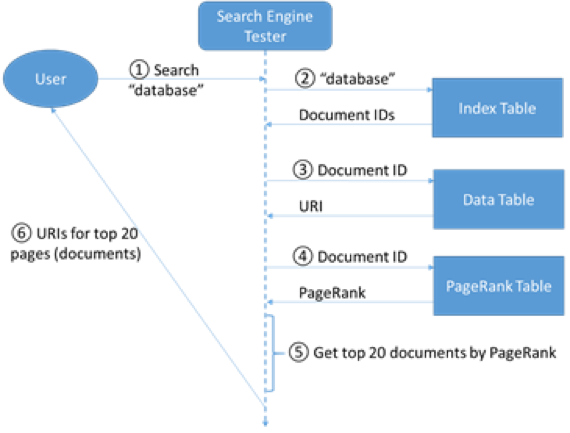
\includegraphics[width=8cm,height=6cm]{p6}
\centering
\caption{Dataflow for searching keyword ``database'' among the constructed databases}
\end{figure}

You need to complete the following code before you can run the search engine:
\begin{lstlisting}[language=bash]
$ vim src/iu/pti/hbaseapp/clueweb09/SearchEngineTester.java
\end{lstlisting}

\lstinputlisting[language=Java]{SearchEngineTester.java}

\section*{Compile and Run the Program}
\begin{lstlisting}[language=bash]
$ cd /root/MoocHomeworks/HBaseInvertedIndexing/
$ vim src/iu/pti/hbaseapp/clueweb09/SearchEngineTester.java
$ cd /root/MoocHomeworks/HBaseInvertedIndexing/
$ ant
$ cp /root/MoocHomeworks/HBaseInvertedIndexing/dist/lib/cglHBaseMooc.jar /root/software/hadoop-1.1.2/lib/
\end{lstlisting}

Now you can test the functionality of the search engine by running the program with keywords.

\begin{lstlisting}[language=bash]
$ cd /root/software/hadoop-1.1.2/
$ ./bin/hadoop jar lib/cglHBaseMooc.jar  iu.pti.hbaseapp.clueweb09.SearchEngineTester search-keyword snapshot
$ ./bin/hadoop jar lib/cglHBaseMooc.jar  iu.pti.hbaseapp.clueweb09.SearchEngineTester get-page-snapshot 00000113548 |  grep snapshot
\end{lstlisting}

\section*{What?s next?}
Congratulations, you have finished the search engine project!

\bibliographystyle{unsrt} 
\end{document}
